Figure \ref{fig:design} shows the architecture of \NAME{}.
% \yifan{Tried to clarify what is taken from existing work vs.~homemade. See if that comes across.}
% \matei{Idea: maybe we can add to the caption of Fig. 1 something like ``Our contributions
%   are shown in color'' or something like that. Or if that's not accurate, outline the boxes
% that we did in some color and make the arrows we did (translations) that color too.}
\NA{The input to \NAME{} is an operator written in TVM's tensor expression (TE) language,
  either directly or converted from PyTorch or TensorFlow layers by TVM Relax~\cite{relax}.
  First, \NAME{}'s auto-scheduler (\S\ref{sec:auto-sched}) finds high-performance schedules
  for the program on the target GPU without user intervention,
  while keeping the program \emph{tile-ready}, i.e., in the regular form tile compilers expect,
  with perfectly nested tile-sized inner loops and no scan dependencies.
  Schedules are written in a scheduling language over the program's \emph{block graph}
  (\S\ref{sec:block-graph}).
  Then, \NAME{} successively lowers the scheduled program from its scalar IR
  through two tile IRs (\S\ref{sec:opt-pipeline}):
  a virtual register tile IR (VR-tile IR) for expression rewriting,
  and a memory access tile IR (MA-tile IR), which \NAME{} translates into the language of
  a tile compiler (Triton, Tawa, or TileLang) that performs tile-level SIMD optimizations
and generates the kernel.}
Besides TE, other tensor expression languages, e.g., JAX's jaxpr,
\mbox{could also serve as \NAME{}'s input.}

\begin{figure}[t]
  \centering
  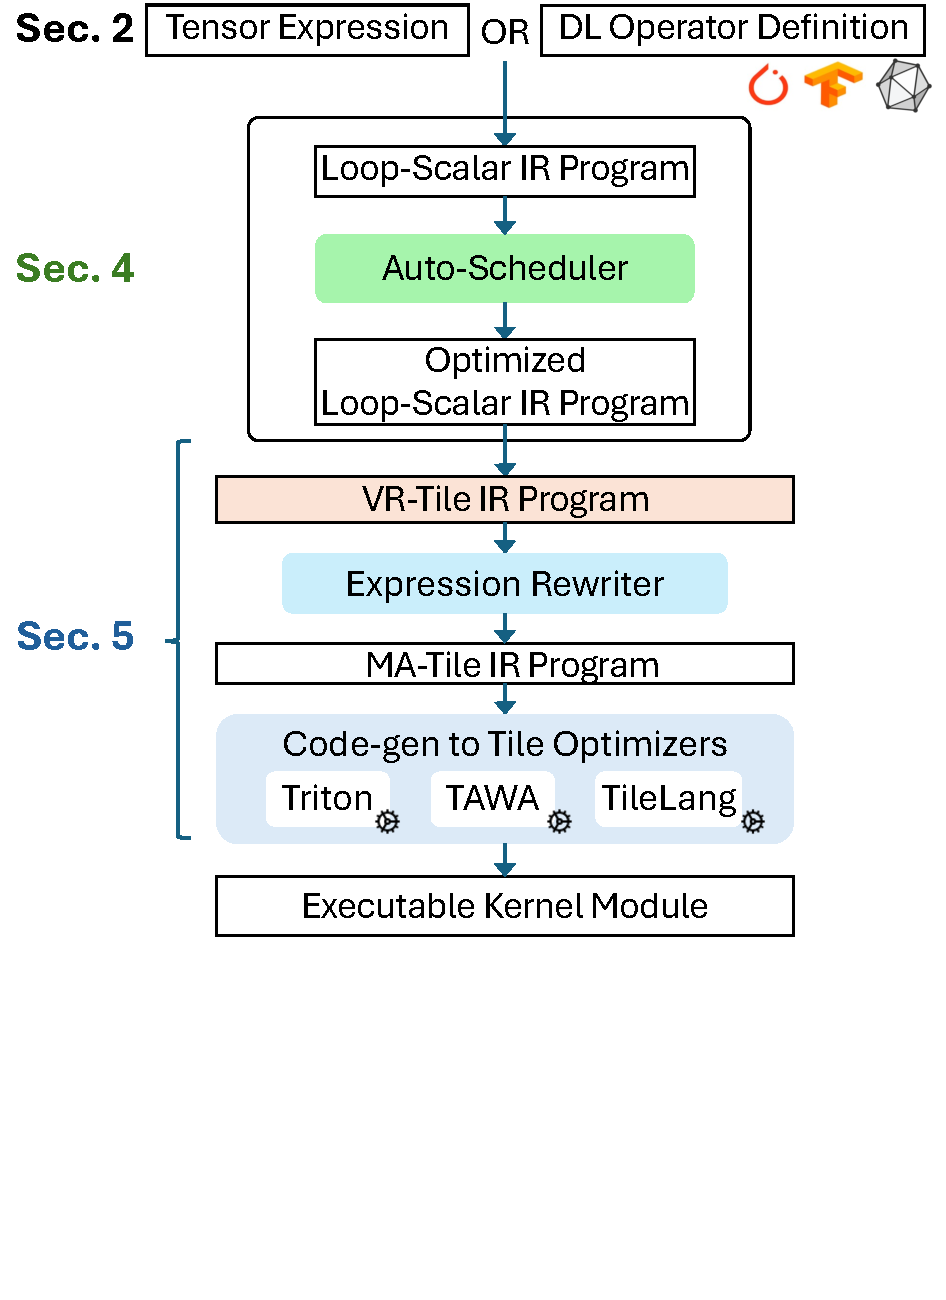
\includegraphics[width=0.8\columnwidth, trim=0mm 61mm 2mm 0mm, clip,
  page=1]{figures/one-col-figs.pdf}
  \vspace{-.05in}
  \caption{System overview of \NAME{}. Novel components from our contributions are shown
  in colored boxes.}
  % \sasa{We should either remove Tiled optimizers box or call it 'Codegen to Tile Optimizers'}}
  \label{fig:design}
\end{figure}

\begin{figure}[t]
  \centering
  \includegraphics[width=0.9\columnwidth, trim=0mm 5mm 25mm 0mm, clip,
  page=2]{figures/one-col-figs.pdf}
  \vspace{-.1in}
  \caption{An example of scheduling a block graph.
    A scalar IR program and its corresponding block graph are shown at the top,
    followed by examples of using scheduling primitives to transform the block graph. In
  this graph, ovals represent \emph{compute statements} and rectangles represent \emph{loops}. }
  \label{fig:sched-example}
\end{figure}

\textbf{Block Graph.}
\label{sec:block-graph}
The block graph is the program representation that \NAME{}'s scheduling manipulates.
It combines the AST of a scalar IR program with its data dependency graph,
\NA{and models the program only down to the granularity of a GPU thread block:
  which loops and statements each block executes, how data flows between statements, and
  where tensors are placed. Lower-level details, such as how a block's tile
  computation maps to warps and threads, are absent from the block graph and left to tile compilers.
  % (unlike TensorIR schedules~\cite{tensorir}, which also bind threads and tensorize).
This keeps schedules high-level and the auto-scheduler's search space small.}
The top part of Figure \ref{fig:sched-example} shows an example scalar IR program
(extracted from the attention operator) and its block graph.
Each node corresponds to a \emph{compute statement} in the IR,
and directed edges indicate data dependencies.
The \emph{producers} of a compute statement $n$ are the statements with an edge to $n$,
and $n$ is their \emph{consumer};
\emph{predecessors} and \emph{successors} are \NA{the transitive closures of these relations},
and a \emph{path} from $n_1$ to $n_2$ is a chain of statements, each a producer of the next,
from $n_1$ to $n_2$.
Paths are central to advanced fusion,
which fuses two reductions together with all statements on the path between them
(\S\ref{sec:adv-fusion}).
Boxes around compute statements represent \emph{loops}.
% \matei{term unclear. Intended: spatial/reduction/scan.}
The block graph tracks iteration-carried data dependency of each loop,
determined by the data access pattern of compute statements.
For example, the \texttt{k} loop around the \texttt{mm} node is a reduction loop,
while the loops \texttt{i} and \texttt{j} are map loops.

\NA{\textbf{Scheduling Language.}}
\NAME{}'s scheduling language consists of primitives that transform the block graph
(Table~\ref{tab:primitives} in the appendix).
They cover loop tiling and binding loops to GPU thread blocks,
data placement and caching,
classic loop fusion and advanced reduction fusion (rolling update and split-k update),
and transformations that regularize the program for tile compilers,
such as decomposing reductions and splitting scan buffers.
Many primitives come from TVM and Neptune;
\NAME{} adds primitives for padding axes, folding accumulators, and reordering statements.
The bottom part of Figure~\ref{fig:sched-example} shows examples of applying primitives
to the block graph.
